\documentclass[a4paper,12pt]{article}
\usepackage[utf8]{inputenc}
\usepackage[MeX]{polski}
\usepackage{fixltx2e}
\usepackage[utf8]{inputenc}
\usepackage[T1]{fontenc}
\usepackage{graphicx}
\usepackage{color}
\usepackage{mathtools}
\usepackage{wasysym}
\usepackage[font=small,labelfont=bf]{caption}
\renewcommand*{\tablename}{Tab.}
\renewcommand*{\figurename}{Rys.}
%%%%%%%%%%%%%%%%%%%%%%%%%%%%%%%%%%%%%%%%%%%%%%%%%%%%%%%%%%%%%%%%%%%%%%%%%%%%%%%%%%%%%%%%%%%%%%%%%%%%%%%%%%%%%%%%%%%%%%%%%%%%%%%%%%%%%%%%%%%%%%%%%%%%
%%%%%%%%%%%%%%%%%%%%%%%%%%%%%%%%%%%%%%%%%%%%%%%%%%%%%%%%%%%%%STRONA TYTULOWA%%%%%%%%%%%%%%%%%%%%%%%%%%%%%%%%%%%%%%%%%%%%%%%%%%%%%%%%%%%%%%%%%%%%%%%%
%%%%%%%%%%%%%%%%%%%%%%%%%%%%%%%%%%%%%%%%%%%%%%%%%%%%%%%%%%%%%%%%%%%%%%%%%%%%%%%%%%%%%%%%%%%%%%%%%%%%%%%%%%%%%%%%%%%%%%%%%%%%%%%%%%%%%%%%%%%%%%%%%%%%
\title{\Huge \textbf{Politechnika Wrocławska\\[0.3in]} 
  \huge Katedra Teorii Pola, Układów elektronicznych i Optoelektronicznych \\[0.2in]
  \LARGE Zespół Układów Elektronicznych
}
\date{}
\author{}

\begin{document}
\maketitle

\begin{table}[h]
  \large
  \centering
  \begin{tabular}{|ll|l|}
    \hline
    \multicolumn{1}{|l|}{Data: 12.05.2015r}                & \multicolumn{2}{l|}{Dzień: Wtorek}                                     \\ \hline
    \multicolumn{1}{|l|}{Grupa: VII}                      & \multicolumn{2}{l|}{Godzina: 12:15-15:00}                              \\ \hline
    \multicolumn{3}{|l|}{\textit{\begin{tabular}[c]{@{}l@{}}\textbf{Temat ćwiczenia:} \\ Generatory kwarcowe\end{tabular}}}        \\ \hline
    \textbf{Dane projektowe:}                             & \multicolumn{2}{l|}{}                                                  \\ 
    Rezonator kwarcowy 8.000 MHz                          & \multicolumn{2}{l|}{}                                                                        \\ \hline
    \multicolumn{1}{|l|}{\textbf{l.p}}                    & \textbf{Nazwisko i imię}                 & \textbf{Oceny}              \\ \hline
    \multicolumn{1}{|l|}{1}                               & Arkadiusz Ziółkowski                     &                             \\ \hline
    \multicolumn{1}{|l|}{2}                               & Jakub Koban                              &                             \\ \hline
  \end{tabular}
\end{table}
%%%%%%%%%%%%%%%%%%%%%%%%%%%%%%%%%%%%%%%%%%%%%%%%%%%%%%%%%%%%%%%%%%%%%%%%%%%%%%%%%%%%%%%%%%%%%%%%%%%%%%%%%%%%%%%%%%%%%%%%%%%%%%%%%%%%%%%%%%%%%%%%%%%%
%%%%%%%%%%%%%%%%%%%%%%%%%%%%%%%%%%%%%%%%%%%%%%%%%%%%%%%%%%%%%%%%%%%ZADANIE PROJEKTOWE%%%%%%%%%%%%%%%%%%%%%%%%%%%%%%%%%%%%%%%%%%%%%%%%%%%%%%%%%%%%%%%
%%%%%%%%%%%%%%%%%%%%%%%%%%%%%%%%%%%%%%%%%%%%%%%%%%%%%%%%%%%%%%%%%%%%%%%%%%%%%%%%%%%%%%%%%%%%%%%%%%%%%%%%%%%%%%%%%%%%%%%%%%%%%%%%%%%%%%%%%%%%%%%%%%%%
\pagebreak
\section{Zadanie projektowe}
Zaprojektować:
\begin{enumerate}
\item {Generator kwarcowy Colpittsa-Pierce'a z tranzysotrem bipolarnym :}
  \begin{itemize}
  \item R\textsubscript{1} = 218.75 $k\Omega$
  \item R\textsubscript{2} = 0.9578 $k\Omega$
  \item C\textsubscript{1} = 33 pF
  \item C\textsubscript{2} = 3.3 nF
  \end{itemize}
\item {Generator kwarcowy zrealizowany na bramkach TTL :}
  \begin{itemize}
  \item R\textsubscript{5} = 560 $\Omega$
  \item R\textsubscript{6} = 1.8 $k\Omega$
  \item R\textsubscript{7} = 220 $\Omega$
  \item R\textsubscript{8} = 220 $k\Omega$
  \end{itemize}
\item{Generator kwarcowy realizowany na inwerterach CMOS :}
  \begin{itemize}
  \item R\textsubscript{9} = 10 $M\Omega$
  \item C\textsubscript{5} = 33 pF
  \item C\textsubscript{6} = 33 pF
  \end{itemize}
\item{Zasilanie :}
  \begin{itemize}
  \item C\textsubscript{7} = 33 pF
  \item C\textsubscript{8} = 33 pF
  \end{itemize}
\item Rezonator kwarcowy 8.000 MHz
\end{enumerate}
\pagebreak
%%%%%%%%%%%%%%%%%%%%%%%%%%%%%%%%%%%%%%%%%%%%%%%%%%%%%%%%%%%%%%%%%%%%%%%%%%%%%%%%%%%%%%%%%%%%%%%%%%%%%%%%%%%%%%%%%%%%%%%%%%%%%%%%%%%%%%%%%%%%%%%%%%%%
%%%%%%%%%%%%%%%%%%%%%%%%%%%%%%%%%%%%%%%%%%%%%%%%%%%%%%%%%%%%%%%%%%%CZĘŚĆ PROJEKTOWA%%%%%%%%%%%%%%%%%%%%%%%%%%%%%%%%%%%%%%%%%%%%%%%%%%%%%%%%%%%%%%%%%
%%%%%%%%%%%%%%%%%%%%%%%%%%%%%%%%%%%%%%%%%%%%%%%%%%%%%%%%%%%%%%%%%%%%%%%%%%%%%%%%%%%%%%%%%%%%%%%%%%%%%%%%%%%%%%%%%%%%%%%%%%%%%%%%%%%%%%%%%%%%%%%%%%%%
\section {Schematy projektowy}
%%%%%%%%%%%%%%%%%%%%%%%%%%%%%%%%%%%%%%%%%%%%%%%%%%%%%%%%%%%%%%%%%%%%%%%%%%%%%%%%%%%%%%%%%%%%%%%%%%%%%%%%%%%%%%%%%%%%%%%%%%%%%%%%%%%%%%%%%%%%%%%%%%%%
\begin{center}
  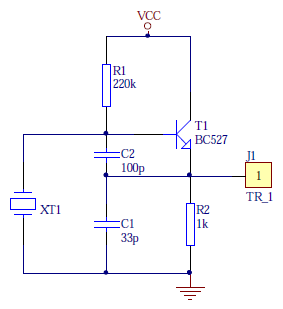
\includegraphics[width=0.5\textwidth]{u1}
  \captionof{figure}{Schemat generatora Colpittsa-Pierce'a }
\end{center}
%%%%%%%%%%%%%%%%%%%%%%%%%%%%%%%%%%%%%%%%%%%%%%%%%%%%%%%%%%%%%%%%%%%%%%%%%%%%%%%%%%%%%%%%%%%%%%%%%%%%%%%%%%%%%%%%%%%%%%%%%%%%%%%%%%%%%%%%%%%%%%%%%%%%
\begin{center}
  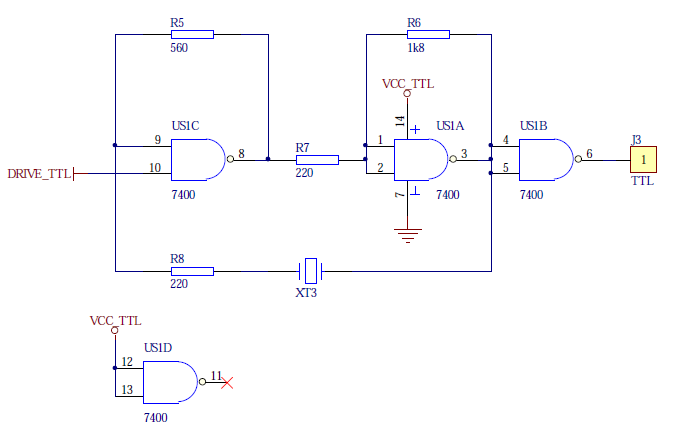
\includegraphics[width=0.65\textwidth]{u2} 
  \captionof{figure}{Schemat generatora na bramkach TTL  }
\end{center}
%%%%%%%%%%%%%%%%%%%%%%%%%%%%%%%%%%%%%%%%%%%%%%%%%%%%%%%%%%%%%%%%%%%%%%%%%%%%%%%%%%%%%%%%%%%%%%%%%%%%%%%%%%%%%%%%%%%%%%%%%%%%%%%%%%%%%%%%%%%%%%%%%%%%
\begin{center}
  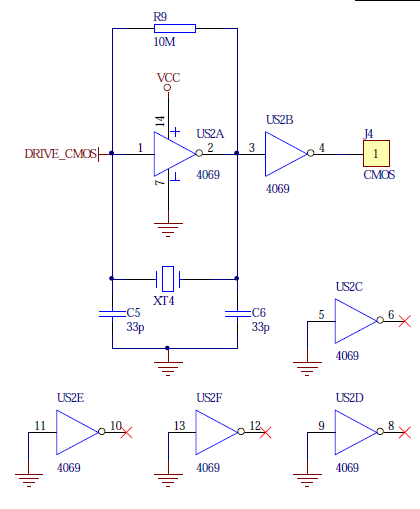
\includegraphics[width=0.6\textwidth]{u3}
  \captionof{figure}{Schemat generatora na inwerterach CMOS  }
\end{center}
%%%%%%%%%%%%%%%%%%%%%%%%%%%%%%%%%%%%%%%%%%%%%%%%%%%%%%%%%%%%%%%%%%%%%%%%%%%%%%%%%%%%%%%%%%%%%%%%%%%%%%%%%%%%%%%%%%%%%%%%%%%%%%%%%%%%%%%%%%%%%%%%%%%%
%%%%%%%%%%%%%%%%%%%%%%%%%%%%%%%%%%%%%%%%%%%%%%%%%%%%%%%%%%%%%%%%%%%CZĘŚĆ LABORATORYJNA%%%%%%%%%%%%%%%%%%%%%%%%%%%%%%%%%%%%%%%%%%%%%%%%%%%%%%%%%%%%%%
%%%%%%%%%%%%%%%%%%%%%%%%%%%%%%%%%%%%%%%%%%%%%%%%%%%%%%%%%%%%%%%%%%%%%%%%%%%%%%%%%%%%%%%%%%%%%%%%%%%%%%%%%%%%%%%%%%%%%%%%%%%%%%%%%%%%%%%%%%%%%%%%%%%%
\section{Część laboratoryjna}\
%%%%%%%%%%%%%%%%%%%%%%%%%%%%%%%%%%%%%%%%%%%%%%%%%%%%%%%%%%%%%%%%%%%%%%%%%%%%%%%%%%%%%%%%%%%%%%%%%%%%%%%%%%%%%%%%%%%%%%%%%%%%%%%%%%%%%%%%%%%%%%%%%%%%
\subsection{Generator Colpittsa-Pierce'a }
\\ \\
\begin{center}
  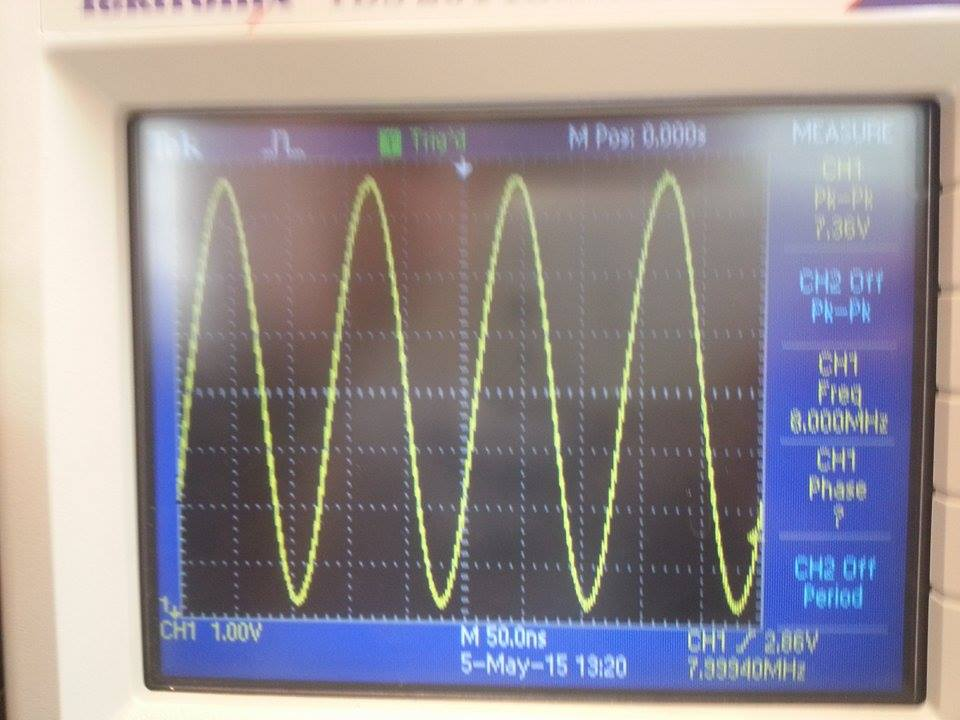
\includegraphics[width=0.5\textwidth]{o3}
  \captionof{figure}{Przebieg generowanego sygnału}
\end{center}


\begin{table}[h]}
    \centering
    \captionof{table}{Wyniki pomiarów napięcia zasilania U oraz częstotliwośći f generowanego sygnału}
    \begin{tabular}{|c|c|c|} \hline
      \textbf{U {[}V{]}} & \textbf{f {[}MHz{]}} & \textbf{Odchylenie {[\permil]}} \\ \hline
      9         & 7.99934     & -0.082                 \\ \hline
      10        & 7.99935     & -0.081                 \\ \hline
      10.5      & 7.99935     & -0.081                 \\ \hline
      11        & 7.99936     & -0.080                 \\ \hline
      11.5      & 7.99936     & -0.080                 \\ \hline
      12        & 7.99937     & -0.079                 \\ \hline
      12.5      & 7.99937     & -0.079                 \\ \hline
      13        & 7.99938     & -0.077                 \\ \hline
      13.5      & 7.99938     & -0.077                 \\ \hline
      14        & 7.99939     & -0.076                 \\ \hline
      14.5      & 7.99939     & -0.076                 \\ \hline
      15        & 7.99940     & -0.075                 \\ \hline
    \end{tabular}
\end{table}

\begin{center}
  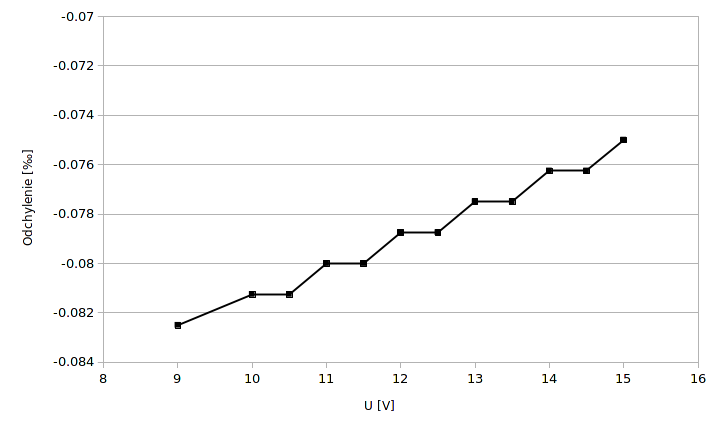
\includegraphics[width=1\textwidth]{z3}
  \captionof{figure}{Zależność odchylenia częstotliwości (od wartości nominalnej 8.000 MHz) od napięcia zasilania  }
\end{center}

Układ rozpoczął poprawną pracę od napięcia zasilania 9 V. Wraz ze wzrostem napięcia zmniejsza się odchylenie częstotliwości generowanego sygnału od wartościu zadanej (8.000 MHz). Maksymalne odchylenie od wartości nominalnej wynosi 0.082\permil. Generowany sygnał jest sinusoidalny.
%%%%%%%%%%%%%%%%%%%%%%%%%%%%%%%%%%%%%%%%%%%%%%%%%%%%%%%%%%%%%%%%%%%%%%%%%%%%%%%%%%%%%%%%%%%%%%%%%%%%%%%%%%%%%%%%%%%%%%%%%%%%%%%%%%%%%%%%%%%%%%%%%%%%
\subsection{Generator realizowany na bramkach TTL }
\\
\\
\begin{center}
  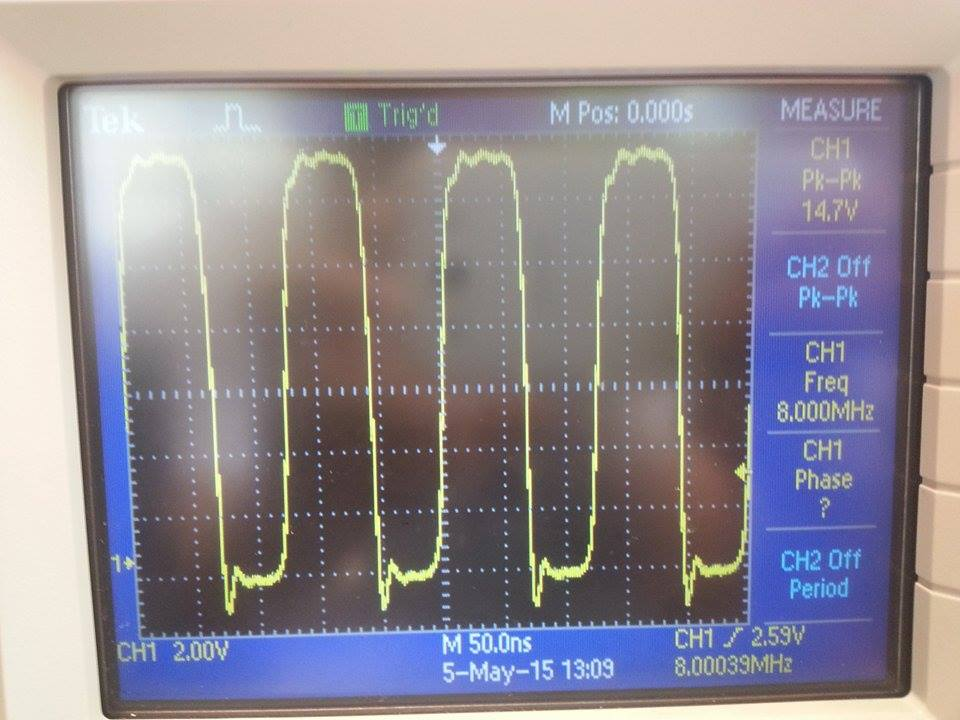
\includegraphics[width=0.5\textwidth]{o1} 
  \captionof{figure}{Przebieg generowanego sygnału}
\end{center}
\\
\begin{table}[h]
  \captionof{table}{Wyniki pomiarów napięcia zasilania U oraz częstotliwośći f generowanego sygnału }
  \centering
\begin{tabular}{|c|c|c|}
\hline
\textbf{U {[}V{]}} & \textbf{f {[}MHz{]}} & \textbf{Odchylenie {[\permil]}} \\ \hline
2.8                & 7.99827              & -0.216                     \\ \hline
3                  & 7.99861              & -0.174                     \\ \hline
3.3                & 7.99886              & -0.142                     \\ \hline
3.6                & 7.99896              & -0.130                     \\ \hline
3.9                & 7.99899              & -0.126                     \\ \hline
4.1                & 7.99899              & -0.126                     \\ \hline
4.3                & 7.99894              & -0.132                     \\ \hline
4.5                & 7.99896              & -0.130                     \\ \hline
4.7                & 7.99896              & -0.130                     \\ \hline
5                  & 7.99892              & -0.135                     \\ \hline
\end{tabular}
\end{table}

\begin{center}
  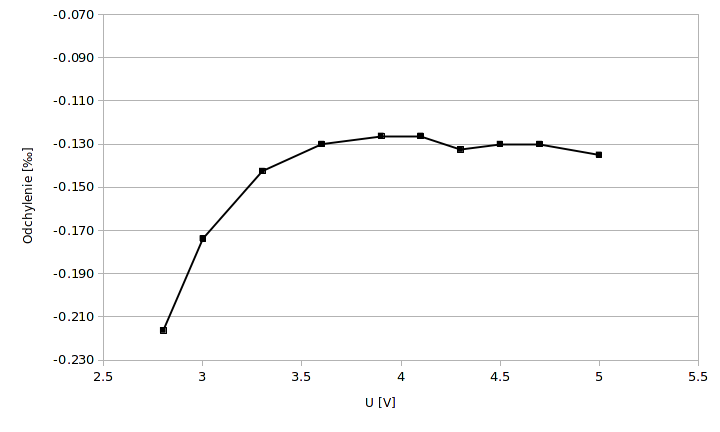
\includegraphics[width=1\textwidth]{z1}
  \captionof{figure}{Zależność odchylenia częstotliwości (od wartości nominalnej 8.000 MHz) od napięcia zasilania}
\end{center}
Układ rozpoczął poprawną pracę od napięcia zasilania 2.8 V. Wraz ze wzrostem napięcia zmniejsza się odchylenie częstotliwości generowanego sygnału od wartościu zadanej (8.000 MHz). Maksymalne odchylenie od wartości nominalnej wynosi 0.216\permil. Generowany sygnał przypomina prostokątny.

\pagebreak
%%%%%%%%%%%%%%%%%%%%%%%%%%%%%%%%%%%%%%%%%%%%%%%%%%%%%%%%%%%%%%%%%%%%%%%%%%%%%%%%%%%%%%%%%%%%%%%%%%%%%%%%%%%%%%%%%%%%%%%%%%%%%%%%%%%%%%%%%%%%%%%%%%%%
\subsection{Generator realizowany na inwerterach CMOS }
\begin{center}
  \center
  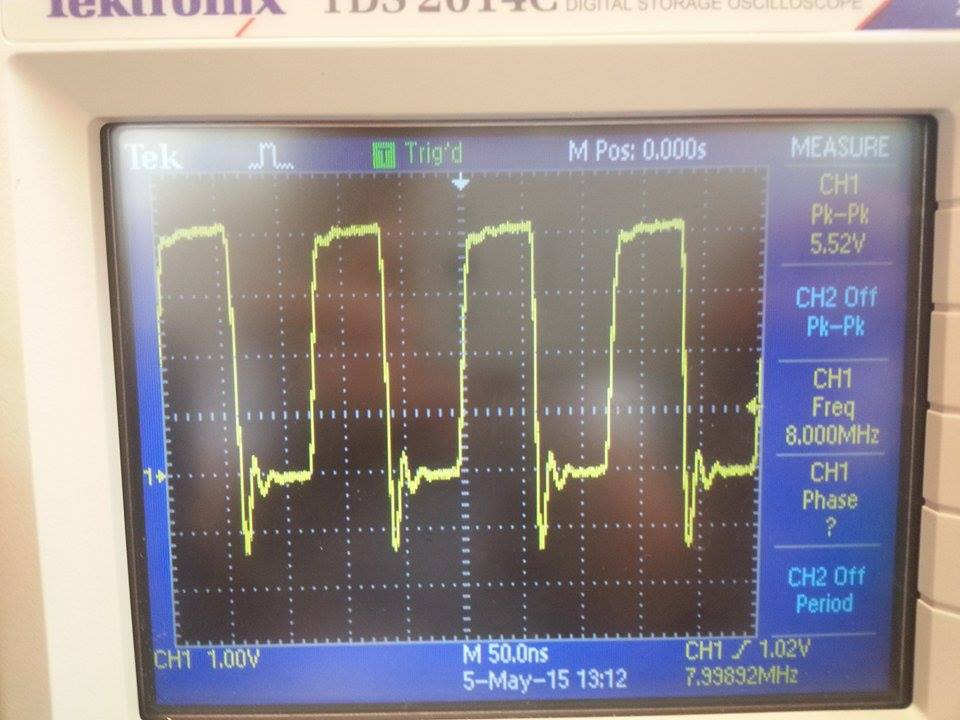
\includegraphics[width=0.5\textwidth]{o2}
  \captionof{figure}{Przebieg generowanego sygnału}
\end{center}

\begin{table}[h]
  \captionof{table}{Wyniki pomiarów napięcia zasilania U oraz częstotliwośći f generowanego sygnału}
  \centering
  \begin{tabular}{|c|c|c|}
\hline
\textbf{U {[}V{]}} & \textbf{f {[}MHz{]}} & \textbf{Odchylenie {[\permil]}} \\ \hline
5                  & 8.00035              & 0.044                      \\ \hline
5.5                & 8.00035              & 0.044                      \\ \hline
6                  & 8.00035              & 0.044                      \\ \hline
6.5                & 8.00035              & 0.044                      \\ \hline
7                  & 8.00035              & 0.044                      \\ \hline
7.5                & 8.00035              & 0.044                      \\ \hline
8                  & 8.00036              & 0.045                      \\ \hline
8.5                & 8.00036              & 0.045                      \\ \hline
9                  & 8.00036              & 0.045                      \\ \hline
9.5                & 8.00036              & 0.045                      \\ \hline
10                 & 8.00037              & 0.046                      \\ \hline
10.5               & 8.00038              & 0.047                      \\ \hline
11                 & 8.00039              & 0.049                      \\ \hline
11.5               & 8.00039              & 0.049                      \\ \hline
12                 & 8.00039              & 0.049                      \\ \hline
12.5               & 8.00040              & 0.050                      \\ \hline
13                 & 8.00040              & 0.050                      \\ \hline
13.5               & 8.00041              & 0.051                      \\ \hline
14                 & 8.00041              & 0.051                      \\ \hline
14.5               & 8.00042              & 0.053                      \\ \hline
15                 & 8.00042              & 0.053                      \\ \hline
\end{tabular}
\end{table} 

\begin{center}
  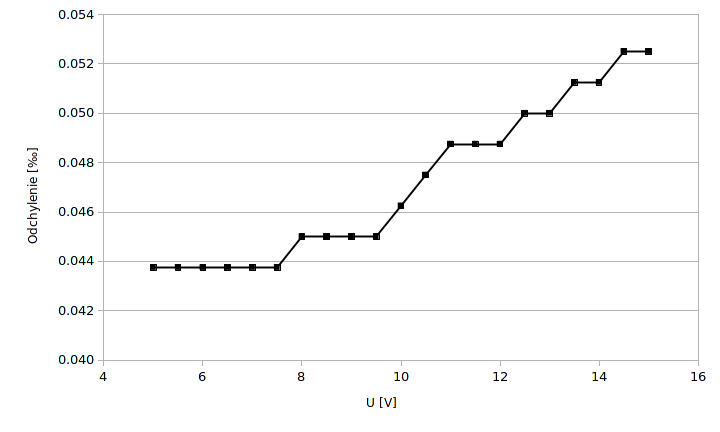
\includegraphics[width=1\textwidth]{z2}
  \captionof{figure}{Zależność odchylenia częstotliwości (od wartości nominalnej 8.000 MHz) od napięcia zasilania}
\end{center}
Układ rozpoczął poprawną pracę od napięcia zasilania 5 V. Wraz ze wzrostem napięcia zwiększa się odchylenie częstotliwości generowanego sygnału od wartościu zadanej (8.000 MHz). Maksymalne odchylenie od wartości nominalnej wynosi 0.053\permil. Generowany sygnał przypomina prostokątny.
\section {Wnioski}
\begin{enumerate}
\item Wszystkie generatory pozwalają na realizowanie swojej funkcji z bardzo dużą dokładnością. Najmniejszym odchyleniem od wartości zadanej (8.000 MHz) cechuje się generator zrealizowany w oparciu o inwertery CMOS (0.053\permil).
\item Generator Colpittsa-Pierce'a generuje sygnał sinusoidalny.
\item Sygnały z generatorów opartych na bramkach TTL oraz inwerterach CMOS są prostokątne z uwagi na cyfrowe bramki logiczne zastosowane do ich budowy.
\end{enumerate}
\end{document}
